\documentclass[10pt,a4paper]{article} 
\fontfamily{cmss}
\usepackage{amsmath}
\usepackage{amssymb}
\usepackage{mathtools}
\usepackage[brazilian]{babel}
\usepackage[utf8]{inputenc}
\usepackage[T1]{fontenc}
\usepackage[parfill]{parskip}
\usepackage[margin=1.0in]{geometry}
\usepackage{graphicx}
\usepackage{type1ec}
\usepackage{graphicx}
\usepackage{listings}
\usepackage[Algoritmo]{algorithm}
\usepackage[noend]{algpseudocode}
\usepackage{booktabs}
\usepackage{multirow,tabularx}

\usepackage{makecell}
\renewcommand\theadalign{tc}
\renewcommand\theadfont{\bfseries}
\renewcommand\theadgape{\Gape[4pt]}
\renewcommand\cellgape{\Gape[4pt]}

\begin{document}

	% CABECALHO %

	\begin{minipage}[b]{0.05\linewidth}
		
\includegraphics[scale=0.3]{ufmg}
	\end{minipage}
	\hfill
	\begin{minipage}[b]{0.95\linewidth}
		\begin{flushright}
			\textbf{UNIVERSIDADE FEDERAL DE MINAS GERAIS} \\
			\textsc{Graduação em Engenharia de Sistemas} \\
			\textbf{Algoritmos e Estruturas de Dados III - Trabalho Prático 1} \\
			Mortal Kontest \\
			Matheus Silva Araujo - 2013066265
		\end{flushright}
	\end{minipage}

	\begin{center}
		\hrulefill
	\end{center}

	% CABECALHO %

	\section{Introdução}

	No Trabalho Prático 1 da disciplina de Algoritmos e Estruturas de Dados III, o adolescente peculiar Nubby tem um novo problema e quer usar \emph{Programação Dinâmica} para resolvê-lo.

	Nubby e seus amigos irão jogar um campeonato de \emph{Mortal Kontest}, e Nubby possui as probabilidades de vitória e derrota para cada confronto possível entre seus amigos.

	No campeonato, dois participantes são sorteados para jogar a primeira rodada \footnote{As chances de sorteio de cada jogador são sempre as mesmas.}. O competidor que perder é eliminado do campeonato e não volta mais a jogar. O vencedor continua na competição. Um novo participante é sorteado; eles jogam e o vencedor dessa nova rodada continua jogando. O campeonato prossegue assim até que haja apenas dois competidores na última rodada, o que vencer essa partida é declarado campeão.

	Dadas as probabilidades de vitória e derrota de cada confronto, Nubby deseja saber quais são as chances que cada competidor tem de ser o campeão.

	\section{Solução do Problema}

	A ideia inicial para a resolução do problema é que, em um cenário onde $n=4$ e os jogadores são $A$, $B$, $C$ e $D$, a probabilidade de $A$ ser o campeão depende das probabilidades das três possíveis \textit{finais}: $AB$, $AC$ e $AD$.

	$A$ é o campeão quando $B$, $C$ ou $D$ \emph{perdem} essas \textit{finais}.

	Para que a final $AB$ aconteça, é necessário que na rodada anterior estejam $ABC$ ou $ABD$. Ou seja, $AB$ depende da probabilidade de que $C$ perca numa segunda rodada onde há $ABC$ ou que $D$ perca numa segunda rodada com $ABD$.

	A probabilidade de um jogador perder em uma rodada é o somatório das probabilidades de uma partida acontecer multiplacando a probabilidade que o jogador tem de perder essa partida.

	$ABC$ e $ABD$ dependem - por consequência - de $ABCD$ que tem probabilidade $P(ABCD) = 1$.

	Por indução, percebe-se que a probabilidade de um subconjunto $S$, $|S|=i$ é função das probabilidades dos subconjuntos $S'$, $|S'|=i+1$ que originam $S$.

	Portanto, calcular a probabilidade de um conjunto $S'$ é um subproblema para calcular a probabilidade do subconjunto $S$.

	Ainda para o exemplo $n=4$, no momento de calcular a probabilidade de $B$, ela dependerá das probabilidade $AB$, $BC$ e $BD$, no entanto, a probabilidade de $AB$ já foi calculada quando a probabilidade de $A$ foi calculada, portanto há a \textbf{memorização} dos cálculos. Tornando o algoritmo dinâmico mais performático do que uma abordagem de força bruta, por exemplo.

	Para o cálculo de $C$, a memorização terá sido ainda maior. No cálculo de $D$, apenas um cálculo será feito.

	As Figuras \ref{fig_memorizacao1} e \ref{fig_memorizacao2} exemplificam esse processo de memorização.

	\begin{figure}[H]
		\centering
		\caption{Memorização em $P(A)$ e $P(B)$}
		\label{fig_memorizacao1}
		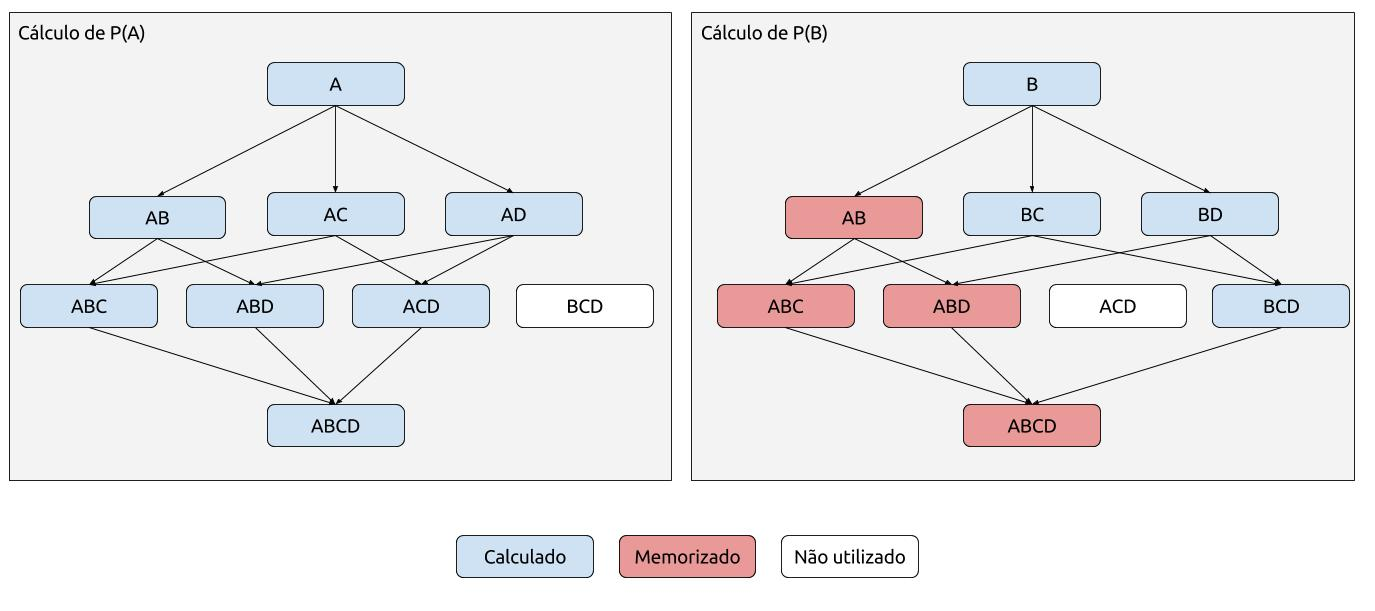
\includegraphics[scale=0.34]{diagrama_n4_a_b}
	\end{figure}

	\begin{figure}[H]
		\centering
		\caption{Memorização em $P(C)$ e $P(D)$}
		\label{fig_memorizacao2}
		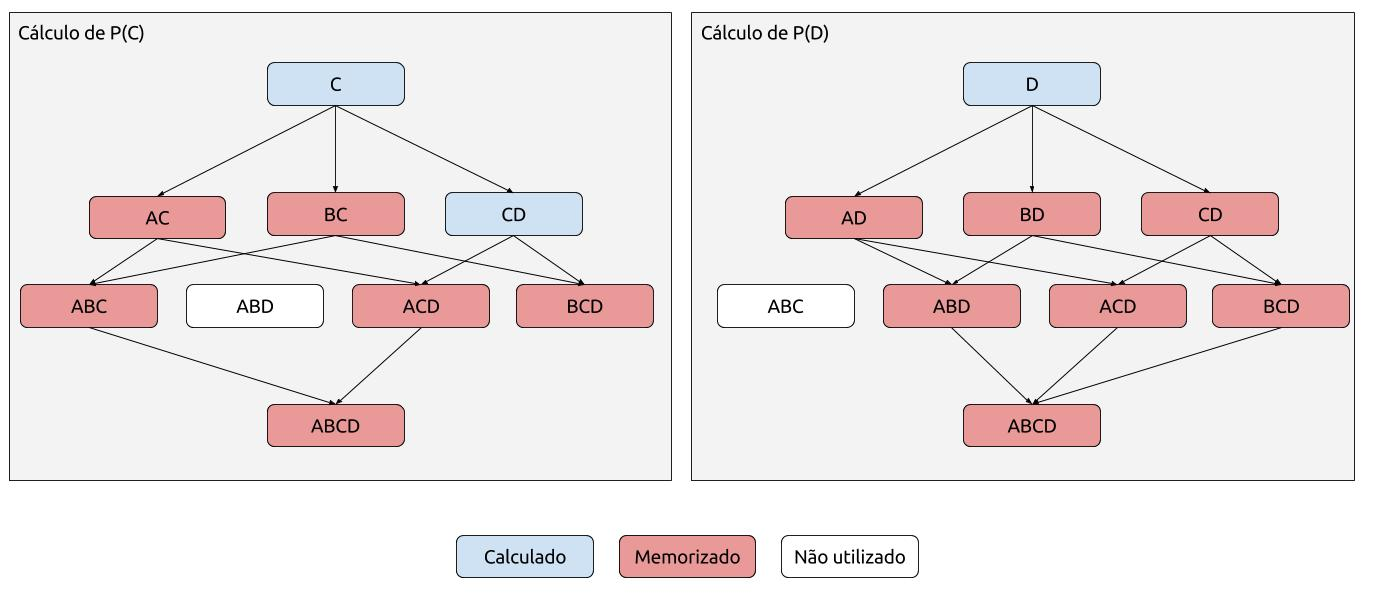
\includegraphics[scale=0.34]{diagrama_n4_c_d}
	\end{figure}

	\subsection{Equação de Recorrência}

	A equação de recorrência para o problema é:

	$$ {P(S)} = P_j(|S'|) \times \sum_{i \notin S} \Big( P(S') \times \sum_{j \in S'} P(j \bigtriangledown i) \Big) $$

	Onde: 

	\begin{itemize}

		\item $S'$ é um conjunto que originou $S$ tendo apenas um elemento $i$ removido

		\item $P_j(|S'|)$ é a probabilidade de um jogo no conjunto $S'$, calculada pela expressão:
		
		$$P_j(|S'|) = \frac{2}{|S'| \times (|S'| - 1)}$$

		\item $P(j \bigtriangledown i)$ é a probabilidade de um jogador $j$ vencer o jogador $i$.

	\end{itemize}

	\section{Análise de Complexidade}

	Com o algoritmo de \emph{Programação Dinâmica} apresentado, a probabilidade de cada subconjunto possível é calculada apenas uma vez, devivo à memorização. Existem $2^n$ subconjuntos possíveis. 

	Para calcular a probabilidade de cada subconjunto há um custo de, no pior caso, $n$ operações. 

	Portanto, a complexidade do algoritmo é de $O(n \cdot 2^n)$. 

    \section{Uso de memória}

    Para armazenar as probabilidades de cada subconjunto é possível utilizar apenas um vetor, cada elemento desse vetor apresenta a probabilidade de um subconjunto, portanto esse vetor tem tamanho $2^n$.

	\section{Avaliação Experimental}

	O algoritmo de \emph{Programação Dinâmica} foi avaliado, e adicionalmente foi feita uma comparação de seu desempenho com um algoritmo de \emph{Força Bruta}.

	\subsection{Algoritmo \emph{Programação Dinâmica}}

	Para avaliar a implementação do algoritmo de \emph{Programação Dinâmica} foram criados 25 casos de teste com $n$ variando de $1$ a $25$ e tomadas as medidas de tempo e uso de memória. Os testes foram feitos em ambiente \emph{Linux Ubuntu}.

	Para medir o tempo, a aplicação foi executada três vezes para cada valor de $n$ e os tempos medidos através do comando \emph{time}.

	Para medir a memória, foi usada a ferramenta \emph{valgrind}.

	A Tabela \ref{tab_tempo} apresenta os valores medidos. Na Figura \ref{fig_tempo} é apresentado um gráfico do tempo em função de $n$. Já na Figura \ref{fig_alocacao} é apresentado um gráfico do uso de memória, os valores da tabela são apresentados em função de $log_2$.

	\begin{table}[H]
		\centering
		\caption{Medidas de tempo e memória.}
		\label{tab_tempo}
		\begin{tabular}{@{}llllll@{}}
			\toprule 
			\thead{$n$} & \thead{T1 (s)} & \thead{T2 (s)} & \thead{T3 (s)} & \thead{T méd. (s)} & \thead{Memória \\ (bytes)} \\ \midrule
			1 & 0.002 & 0.002 & 0.002 & 0.0020 & 5132 \\ 
			2 & 0.002 & 0.002 & 0.002 & 0.0020 & 5152 \\ 
			3 & 0.002 & 0.002 & 0.002 & 0.0020 & 5188 \\ 
			4 & 0.002 & 0.002 & 0.002 & 0.0020 & 5248 \\ 
			5 & 0.002 & 0.003 & 0.002 & 0.0023 & 5348 \\ 
			6 & 0.002 & 0.002 & 0.002 & 0.0020 & 5520 \\ 
			7 & 0.002 & 0.002 & 0.002 & 0.0020 & 5828 \\ 
			8 & 0.002 & 0.002 & 0.001 & 0.0017 & 6400 \\ 
			9 & 0.003 & 0.002 & 0.003 & 0.0027 & 7492 \\ 
			10 & 0.001 & 0.003 & 0.003 & 0.0023 & 9616 \\ 
			11 & 0.004 & 0.004 & 0.004 & 0.0040 & 13796 \\ 
			12 & 0.005 & 0.003 & 0.006 & 0.0047 & 22080 \\ 
			13 & 0.010 & 0.006 & 0.007 & 0.0077 & 38564 \\ 
			14 & 0.015 & 0.016 & 0.015 & 0.0153 & 71440 \\ 
			15 & 0.018 & 0.018 & 0.019 & 0.0183 & 137092 \\ 
			16 & 0.031 & 0.032 & 0.033 & 0.0320 & 268288 \\ 
			17 & 0.062 & 0.061 & 0.062 & 0.0617 & 530564 \\ 
			18 & 0.123 & 0.124 & 0.126 & 0.1243 & 1054992 \\ 
			19 & 0.261 & 0.269 & 0.287 & 0.2723 & 2103716 \\ 
			20 & 0.729 & 0.721 & 0.712 & 0.7207 & 4201024 \\ 
			21 & 1.772 & 1.813 & 1.75 & 1.7783 & 8395492 \\ 
			22 & 4.014 & 3.956 & 3.999 & 3.9897 & 16784272 \\ 
			23 & 8.978 & 8.925 & 9.022 & 8.9750 & 33561668 \\ 
			24 & 18.612 & 18.806 & 19.857 & 19.0917 & 67116288 \\ 
			25 & 41.552 & 40.269 & 41.13 & 40.9837 & 134225348 \\  \bottomrule
		\end{tabular}
	\end{table}

	\begin{figure}[H]
		\centering
		\caption{Medidas de tempo}
		\label{fig_tempo}
		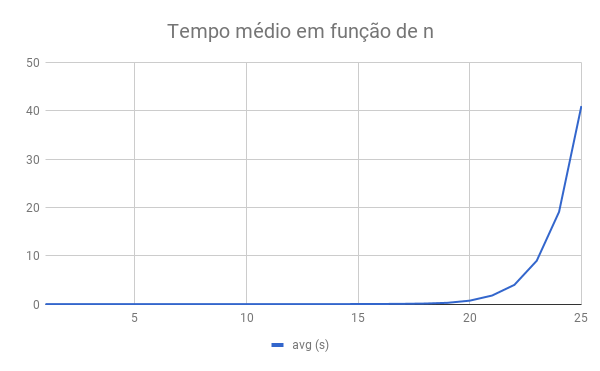
\includegraphics[scale=0.50]{tempo_medio}
	\end{figure}

	\begin{figure}[H]
		\centering
		\caption{Alocação de memória}
		\label{fig_alocacao}
		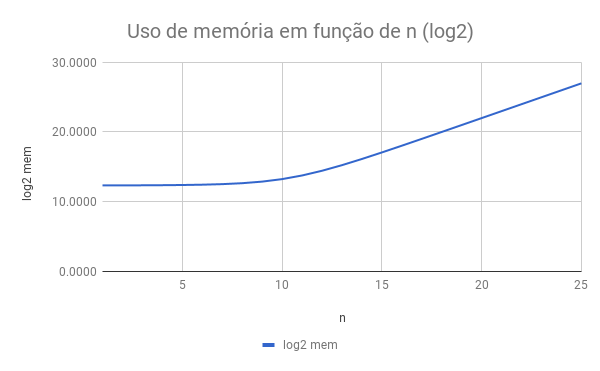
\includegraphics[scale=0.50]{alocacao_memoria}
	\end{figure}

	\subsection{Comparação com \emph{Força Bruta}}

	Durante o desenvolvimento do Trabalho Prático, foi implementado um algoritmo de \emph{Força Bruta} que também resolvia o problema. A fim de comparação, os dois algoritmos foram executados através dos casos de teste \emph{toys} fornecidos e os tempos de execução foram comparados.

	Esse algoritmo \emph{Força Bruta} tem complexidade temporal $O(n!)$.

	Os resultados são apresentados na Tabela \ref{tab_comparacao}, adicionamente um gráfico é apresentado na Figura \ref{fig_comparacao}.

	\begin{table}[H]
		\centering
		\caption{Comparação com algoritmo de \emph{Força Bruta}}
		\label{tab_comparacao}
		\begin{tabular}{@{}lllllllll@{}}
			\toprule 
			& \multicolumn{4}{c}{\thead{\emph{Programação dinâmica}}} & \multicolumn{4}{c}{\thead{\emph{Força Bruta}}} \\
			\thead{$n$} & \thead{T1 (s)} & \thead{T2 (s)} & \thead{T3 (s)} & \thead{T méd. (s)} & \thead{T1 (s)} & \thead{T2 (s)} & \thead{T3 (s)} & \thead{T méd. (s)} \\ \midrule
			1 & 0.002 & 0.002 & 0.002 & 0.0020 & 0.002 & 0.001 & 0.002 & 0.0017 \\ 
			2 & 0.002 & 0.002 & 0.002 & 0.0020 & 0.002 & 0.002 & 0.001 & 0.0017 \\ 
			3 & 0.002 & 0.002 & 0.002 & 0.0020 & 0.002 & 0.002 & 0.002 & 0.0020 \\ 
			4 & 0.002 & 0.002 & 0.002 & 0.0020 & 0.002 & 0.002 & 0.001 & 0.0017 \\ 
			5 & 0.002 & 0.003 & 0.002 & 0.0023 & 0.002 & 0.002 & 0.002 & 0.0020 \\ 
			6 & 0.002 & 0.002 & 0.002 & 0.0020 & 0.002 & 0.001 & 0.002 & 0.0017 \\ 
			7 & 0.002 & 0.002 & 0.002 & 0.0020 & 0.003 & 0.003 & 0.003 & 0.0030 \\ 
			8 & 0.002 & 0.002 & 0.001 & 0.0017 & 0.009 & 0.004 & 0.011 & 0.0080 \\ 
			9 & 0.003 & 0.002 & 0.003 & 0.0027 & 0.031 & 0.036 & 0.035 & 0.0340 \\ 
			10 & 0.001 & 0.003 & 0.003 & 0.0023 & 0.297 & 0.296 & 0.297 & 0.2967 \\   \bottomrule
		\end{tabular}
	\end{table}

	\begin{figure}[H]
		\centering
		\caption{Comparação de algoritmos}
		\label{fig_comparacao}
		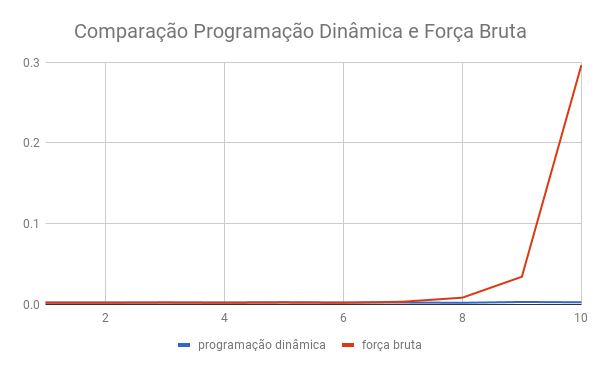
\includegraphics[scale=0.50]{comparacao}
	\end{figure}

	\section{Conclusão}

	Durante a construção do algoritmo e a implementação foi possível notar as vantagens da programação dinâmica. 

	Foi possível sair de um algoritmo com ordem de complexidade temporal de $O(n!)$ para um com $O(n \cdot 2^n)$. 

	Só foi possível \textit{encontrar} o algoritmo \emph{dinâmico} após a implementação do algoritmo \emph{força bruta} e percerber as repetições que permitiam a memorização. O que mostra que algoritmos dinâmicos podem ser entendidos como a combinação de outros algoritmos e memorização.

\end{document}
